\documentclass[10pt,xcolor={x11names}]{beamer}

\usetheme[numbering=fraction,block=fill]{metropolis}
\usecolortheme{seahorse}
\setbeamertemplate{blocks}[rounded]

\usepackage{kmath}
% Tikz
\usetikzlibrary{calc}
\usetikzlibrary{mindmap,trees,shapes,arrows,backgrounds,topaths}
\usetikzlibrary{decorations.pathmorphing, shapes.geometric}

% Text
\usepackage{enumitem}
\usepackage{ulem}
\usepackage{pifont}

% Maths
\usepackage{amsmath}
\usepackage{amsfonts}
\usepackage{amsthm}
\usepackage{amsopn}

% Plots
\usepackage{pgfplots}
\usepgfplotslibrary{groupplots}

% Tables
\usepackage{booktabs}
\usepackage{array}
\newcolumntype{L}{>$l<$}
\arraycolsep=1.4pt
\setlength{\tabcolsep}{3pt}

% Algos
\usepackage[ruled]{algorithm2e}

% Pgfplot
\pgfplotsset{
    legend image code/.code={
        \draw[mark repeat=2,mark phase=2] plot coordinates {
            (0cm,0cm)
            (0.25cm,0cm)
            (0.25cm,0cm)
        };
    }
}
% Objective values and functions
\newcommand{\pobj}{p}
\newcommand{\robj}{r}
\newcommand{\dobj}{d}

% Variables
\newcommand{\pvletter}{x}
\newcommand{\wvletter}{w}
\newcommand{\dvletter}{u}
\newcommand{\vvletter}{v}
\newcommand{\bvletter}{z}
\newcommand{\pv}{\mathbf{\pvletter}}
\newcommand{\wv}{\mathbf{\wvletter}}
\newcommand{\dv}{\mathbf{\dvletter}}
\newcommand{\vv}{\mathbf{\vvletter}}
\newcommand{\bv}{\mathbf{\bvletter}}
\newcommand{\pvi}[1]{\pvletter_{#1}}
\newcommand{\wvi}[1]{\wvletter_{#1}}
\newcommand{\dvi}[1]{\dvletter_{#1}}
\newcommand{\vvi}[1]{\vvletter_{#1}}
\newcommand{\bvi}[1]{\bvletter_{#1}}

% Problem data
\newcommand{\pdim}{n}
\newcommand{\ddim}{m}
\newcommand{\dic}{\mathbf{A}}
\newcommand{\dici}[1]{\mathbf{a}_{#1}}
\newcommand{\dicii}[1]{a_{#1}}
\newcommand{\obs}{\mathbf{y}}
\newcommand{\obsi}[1]{y_{#1}}
\newcommand{\reg}{\lambda}
\newcommand{\groundtruth}{\pv^{\dagger}}
\newcommand{\lfunc}{f}
\newcommand{\pfunc}{h}
\newcommand{\rfunc}{g}
\newcommand{\dfunc}{D}
\newcommand{\relaxrfunc}{\tilde{g}}
\newcommand{\relaxpfunc}{\tilde{h}}
\newcommand{\bigM}{M}
\newcommand{\regtwo}{\alpha}
\newcommand{\rslope}{\tau}
\newcommand{\rlimit}{\mu}
\newcommand{\noise}{\boldsymbol{\epsilon}}

% Indices
\newcommand{\idxentry}{i}

% BnB
\newcommand{\pset}{\mathcal{X}}
\newcommand{\setidx}{\mathcal{S}}
\newcommand{\setzero}{\setidx_0}
\newcommand{\setone}{\setidx_1}
\newcommand{\setnone}{\setidx_\bullet}
\newcommand{\nodeSymb}{\nu}
\newcommand{\node}[1]{#1^{\nodeSymb}}

% Screening
\newcommand{\saferegion}{\mathcal{R}}
\newcommand{\safesphere}{\mathcal{S}}
\newcommand{\spherecenter}{\mathbf{c}}
\newcommand{\sphereradius}{r}

% Peeling
\newcommand{\bigL}{\boldsymbol{\alpha}}
\newcommand{\bigU}{\boldsymbol{\beta}}
\newcommand{\bigLi}[1]{\alpha_{#1}}
\newcommand{\bigUi}[1]{\beta_{#1}}

% Math operators
\DeclareMathOperator{\argmax}{argmax}
\DeclareMathOperator{\argmin}{argmin}
\DeclareMathOperator{\biconjugate}{biconj}
\DeclareMathOperator{\card}{card}
\DeclareMathOperator{\complset}{cmpl}
\DeclareMathOperator{\convex}{cvx}
\DeclareMathOperator{\diam}{diam}
\DeclareMathOperator{\dom}{dom}
\DeclareMathOperator{\interior}{int}
\DeclareMathOperator{\prox}{prox}
\DeclareMathOperator{\rank}{rank}
\DeclareMathOperator{\sign}{sign}


% Math misc
\newcommand{\1}{\mathbf{1}}
\newcommand{\0}{\mathbf{0}}
\newcommand{\abs}[1]{|#1|}
\newcommand{\biconj}[1]{#1^{**}}
\newcommand{\bigO}{\mathcal{O}}
\newcommand{\conj}[1]{#1^{*}}
\newcommand{\icvx}{\eta}
\newcommand{\intervint}[2]{[#1,#2]}
\newcommand{\iter}[2]{#1^{#2}}
\newcommand{\norm}[2]{\|#1\|_#2}
\newcommand{\opt}[1]{#1^{\star}}
\newcommand{\pospart}[1]{[#1]_+}
\newcommand{\separable}[2]{#1_{#2}}
\newcommand{\subdiff}{\partial}
\newcommand{\transp}[1]{#1^{\mathrm{T}}}

% Edition macros
\newcommand{\AddTodo}[1]{\textcolor{red}{[#1]}}

% Colors
\definecolor{Brown}{HTML}{EB811B}
\definecolor{Teal}{HTML}{137D91}
\definecolor{Red}{HTML}{C8412F}
\definecolor{Green}{HTML}{14B03D}

% Beamer elements
\newcommand{\emphcolor}[2]{{\color{#1}#2}}
\newenvironment<>{blockcolor}[2]{%
  \setbeamercolor{block title}{fg=#1,bg=#1!15}%
  \setbeamercolor{block body}{fg=#1,bg=#1!15}%
  \begin{block}#3{\centering#2\par}}{\end{block}}

\title{Tutorial \\ \normalsize{Solving L${}_0$-norm Problems via Mixed-Integer Optimization}}
\date{Simsmart team, Inria Rennes, France \\ 
Applied Mathematics Department, Insa Rennes, France}
\author{\textbf{Théo Guyard}}
\institute{MIND and SODA team seminar \\ October 10th, 2023 \\ Inria Paris Saclay, France}


\begin{document}

\maketitle

\section{Sparse Optimization}

\begin{frame}{Two goals, one problem}
  \begin{tikzpicture}[remember picture,overlay]
    \draw [ultra thick,<->] ($(current page.north)+(-2.2,-0.32\textheight)$) -- ($(current page.north)+(2.2,-0.32\textheight)$) node (arrow) [midway] {};
    \node at ($(arrow.north)+(0,0.1)$) {\textbf{Sparse optimization}};
    \node [text width=0.3\textwidth] at ($(current page.north)+(-4,-0.3\textheight)$) (obs) {
        \begin{blockcolor}{Brown}{}
            \centering
            \textbf{Minimize a function}
        \end{blockcolor}
    };
    \node [text width=.3\textwidth] at ($(current page.north)+(4,-0.3\textheight)$) (dic) {
      \begin{blockcolor}{Brown}{}
            \centering
            \textbf{Sparse solution}
        \end{blockcolor}
    };
    %
    %
    %
    \node at ($(current page.north)+(-2.5,-0.65\textheight)$) (sp) {};
    \node at (sp) {Signal processing};
    \draw ($(sp)+(0,1)$) node {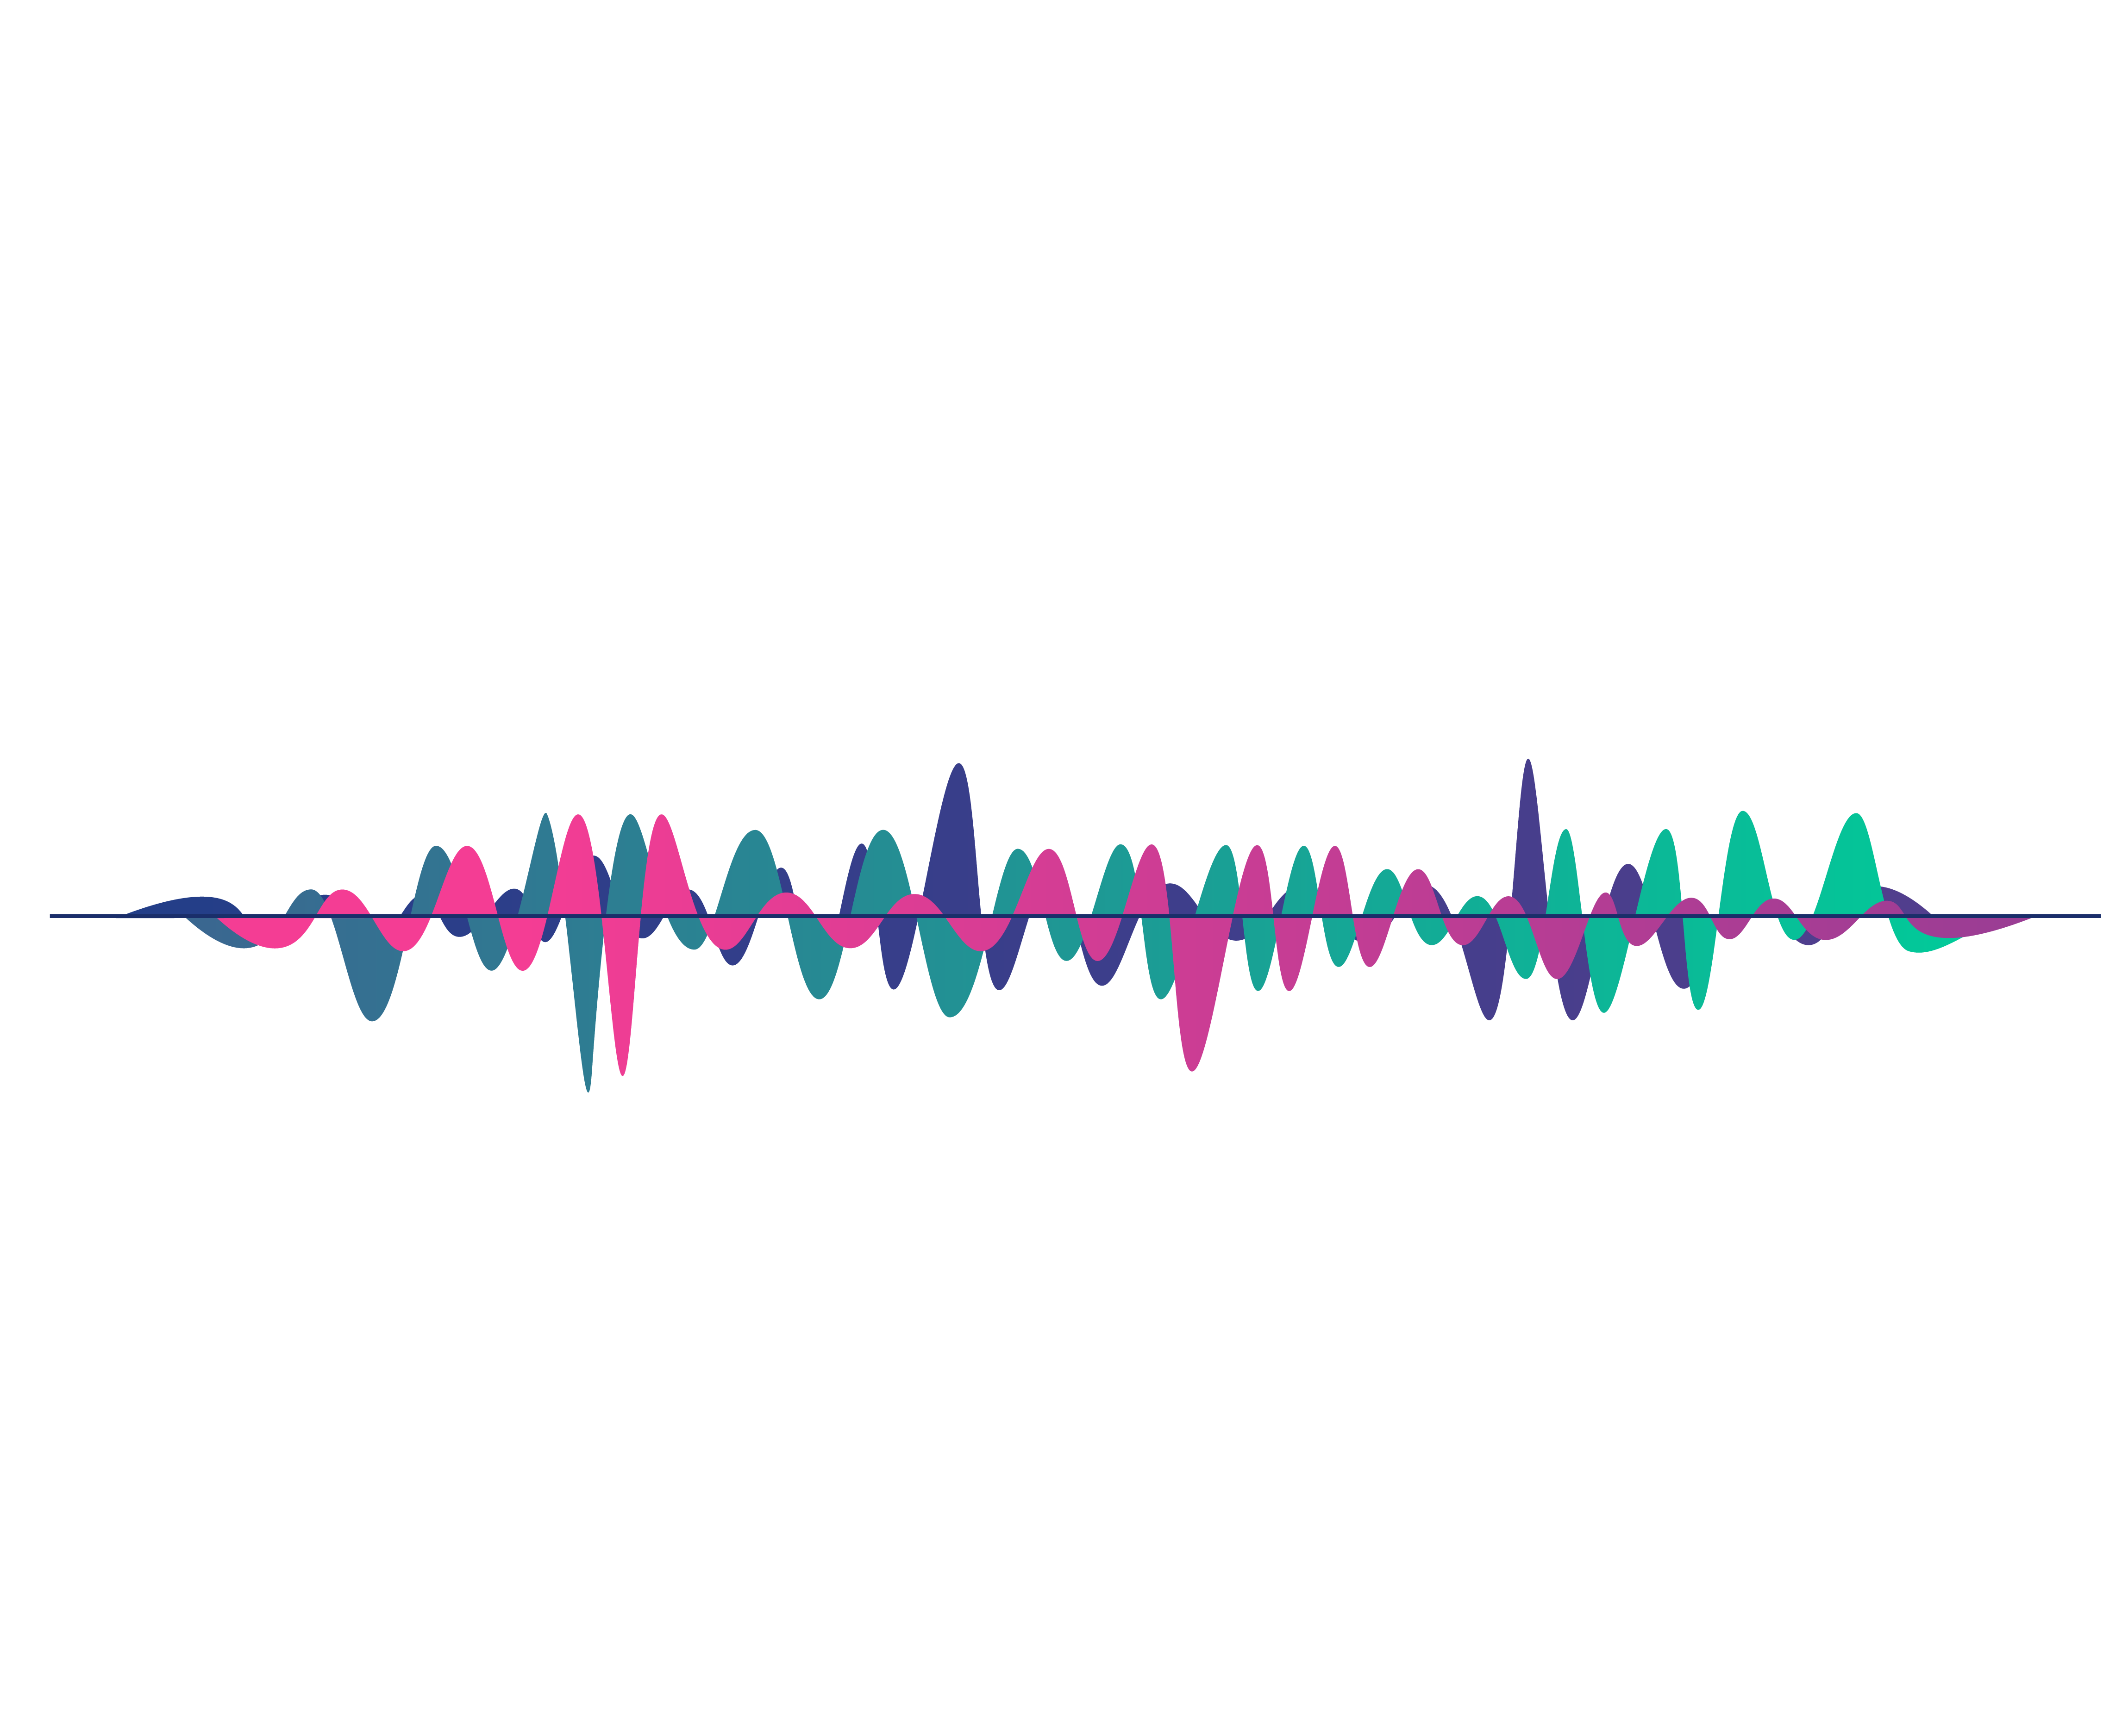
\includegraphics[width=4cm]{imgs/signal-processing.png}};
    %
    %
    %
    \node at ($(current page.north)+(2.5,-0.65\textheight)$) (ml) {};
    \node at (ml) {Machine learning};
    \draw ($(ml)+(0,1)$) node {
\includegraphics[width=2cm]{imgs/machine-learning.png}};
    %
    %
    %
    \node at ($(current page.north)+(-2.5,-0.95\textheight)$) (nd) {};
    \node at (nd) {Network design};
    \draw ($(nd)+(0,1.25)$) node {
\includegraphics[width=1.5cm]{imgs/network.png}};
    %
    %
    %
    \node at ($(current page.north)+(2.5,-0.95\textheight)$) (others) {};
    \node at (others) {And many others};
    \draw ($(others)+(0,1.25)$) node {
\includegraphics[width=1.25cm]{imgs/nerd_face.png}};
  \end{tikzpicture}
\end{frame}

\begin{frame}{Signal processing}
  \begin{tikzpicture}[remember picture,overlay]
    \onslide<+-> {
        \node at ($(current page.north)+(0,-0.2\textheight)$) {\textbf{Compressive sensing}};
        \node (center) at ($(current page.north)+(0,-0.5\textheight)$) {};
        %
        \node (groundtruth) at ($(center)+(-0.4\textwidth,0)$) {$\pv \in \kR^{\pdim}$};
        \node (groundtruth-text) at ($(groundtruth)+(0,0.05\textheight)$) {Sparse signal};
        \node (sensing) at ($(center)+(0,0.175\textheight)$) {Linear measurement through $\dic \in \kR^{\ddim\times\pdim}$};
        \node (observation) at ($(center)+(0.4\textwidth,0)$) {$\obs \in \kR^{\ddim}$};
        \node (observation-text) at ($(observation)+(0,0.05\textheight)$) {Observation};
        \node (recovery) at ($(center)+(0,-0.1\textheight)$) {\emphcolor{Brown}{Recover $\pv$ from $(\dic,\obs)$}};
        \draw [ultra thick,->] ($(groundtruth-text.north east)+(0,0)$) .. controls ($(sensing.south)+(0,0)$) .. ($(observation-text.north west)+(0,0)$);
        \draw [ultra thick,->] ($(observation-text.south west)+(0,0)$) .. controls ($(recovery.north)+(0,0)$) .. ($(groundtruth-text.south east)+(0,0)$);
        %
        %
        %
        \draw ($(groundtruth)+(0,-1)$) node {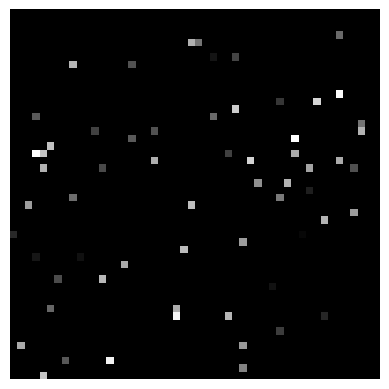
\includegraphics[width=1.5cm]{imgs/cs-x.png}};
        \draw ($(observation)+(0,-1)$) node {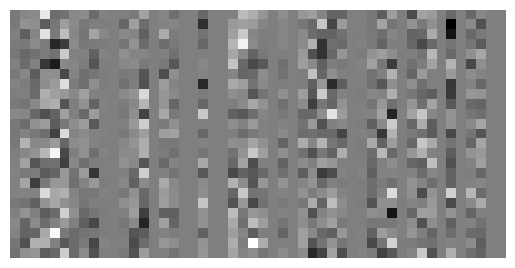
\includegraphics[width=2cm]{imgs/cs-y.png}};
        %
        %
        %
        \node [text width=0.5\textwidth] at ($(center)+(0,-0.3\textheight)$) (problem) {
            \begin{blockcolor}{black}{}
                \centering
                \textbf{Find $\pv$ such that $\obs \simeq \dic\pv$}
            \end{blockcolor}
        };
    }
    %
    %
    %
    \onslide<+-> {
        \node at ($(center)+(0,-0.39\textheight)$) (dimension) {$\ddim \ll \pdim$ : no unique solution};
    }
    %
    %
    %
    \onslide<+-> {
        \node [text width=0.5\textwidth] at ($(center)+(0,-0.3\textheight)$) (problem) {
            \begin{blockcolor}{black}{}
                \centering
                \textbf{Find $\pv$ \emphcolor{Brown}{sparse} such that $\obs \simeq \dic\pv$}
            \end{blockcolor}
        };
    }
  \end{tikzpicture}
\end{frame}

\begin{frame}{Machine learning}
    \begin{tikzpicture}[remember picture,overlay]
        \onslide<+-> {
            \node at ($(current page.north)+(0,-0.35\textheight)$) {
                \begin{tabular}{cccccc}
                    \multicolumn{6}{c}{\textbf{Heart disease dataset (LIBSVM)}} \\
                    \toprule
                    Age & Sex & Cholesterol & Blood pressure & ... & \textbf{Disease} \\
                    \midrule
                    31 & M & 50.3 mg/dl  & 95 mm/hg & ... & \textbf{No} \\
                    35 & F & 54.9 mg/dl & 98 mm/hg & ... & \textbf{Yes} \\
                    42 & F & 49.8 mg/dl & 92 mm/hg & ... & \textbf{Yes} \\
                    37 & M & 59.1 mg/dl & 89 mm/hg & ... & \textbf{No} \\
                    ... & ... & ... & ... & ... & ... \\
                    \bottomrule
                \end{tabular}
            };
        }
        %
        %
        %
        \onslide<+-> {
            \node[align=center,text width=0.2\textwidth] (data) at ($(current page.north)+(-4.5,-0.7\textheight)$) {
                \begin{blockcolor}{black}{}
                    \centering\textbf{Data}
                \end{blockcolor}
            };
            %
            \node[align=center,text width=0.3\textwidth] (logreg) at ($(current page.north)+(0,-0.7\textheight)$) {
                \begin{blockcolor}{black}{Logistic regression}
                    \centering$\min_{\pv} \ \text{LogLoss}(\pv)$
                \end{blockcolor}
            };
            \draw[ultra thick,->] ($(data.east)+(0.1,-0.2)$) -- ($(logreg.west)+(-0.1,-0.2)$);
            %
            \node[align=center,text width=0.2\textwidth] (estimator) at ($(current page.north)+(4.5,-0.7\textheight)$) {
                \begin{blockcolor}{black}{}
                    \centering\textbf{Estimator}
                \end{blockcolor}
            };
            \draw[ultra thick,->] ($(logreg.east)+(0.1,-0.2)$) -- ($(estimator.west)+(-0.1,-0.2)$);
        }
        %
        %
        %
        \onslide<+-> {
            \draw[ultra thick,<-,Brown] ($(estimator.south)+(-0.75,-0)$) .. controls ($(estimator.south)+(-1,-0.5)$) .. ($(estimator.south)+(-1,-1)$) node[below,align=center,text width=0.6\textwidth] {Involves all the features \\ Explainability and robustness issues};
        }
        %
        %
        %
        \onslide<+-> {
            \draw[ultra thick,<-,Brown] ($(logreg.south)+(-1.75,-0)$) .. controls ($(logreg.south)+(-2,-0.5)$) .. ($(logreg.south)+(-2,-1)$) node[below,align=center,text width=0.6\textwidth] {Force the use of only few \\ features via sparsity in $\pv$};
        }
    \end{tikzpicture}
\end{frame}

\begin{frame}{Finance}
    \begin{tikzpicture}[remember picture,overlay]
        \node[align=center,text width=0.45\textwidth] (problem) at ($(current page.north)+(0,-0.4\textheight)$) {
            \begin{blockcolor}{black}{Portfolio selection problem}
                \centering$\left\{\begin{array}{rl}
                    \max & \transp{\mathbf{c}}\pv - \tfrac{\sigma}{2}\transp{\pv}\Sigma\pv \\
                    \text{s.t.} & \transp{1}\pv = 1 \\
                    & \emphcolor{Brown}{\pv \ \text{is k-sparse}}
                \end{array}\right.$
            \end{blockcolor}
        };
        %
        \node[align=center,text width=0.7\textwidth] (xi) at ($(problem)+(1,-0.3\textheight)$) {\begin{itemize}
            \item[$\pvi{\idxentry}$ :] proportion of investment in asset i
            \item[$c_{\idxentry}$ :] profit of asset i
            \item[$\Sigma_{i,j}$ :] covariance of assets i and j
            \item[$k$ :] diversification budget
        \end{itemize}};
    \end{tikzpicture}
\end{frame}

\begin{frame}{Objective, constraint or both ?}
    \begin{tikzpicture}[remember picture,overlay]
        \onslide<+-> {
            \draw [ultra thick,<->] ($(current page.north)+(-2.2,-0.32\textheight)$) -- ($(current page.north)+(2.2,-0.32\textheight)$) node (arrow) [midway] {};
            \node at ($(arrow.north)+(0,0.1)$) {\textbf{Sparse optimization}};
            \node [text width=0.3\textwidth] at ($(current page.north)+(-4,-0.3\textheight)$) (obs) {
                \begin{blockcolor}{Brown}{}
                    \centering
                    \textbf{Minimize a function}
                \end{blockcolor}
            };
            \node at ($(current page.north)+(-4,-0.4\textheight)$) {\emphcolor{Brown}{Loss $\lossfunc(\pv)$}};
            \node [text width=.3\textwidth] at ($(current page.north)+(4,-0.3\textheight)$) {
            \begin{blockcolor}{Brown}{}
                    \centering
                    \textbf{Sparse solution}
                \end{blockcolor}
            };
            \node at ($(current page.north)+(4,-0.4\textheight)$) {\emphcolor{Brown}{Counting function $\norm{\pv}{0}$}};
        }
        %
        %
        %
        \onslide<+-> {
            \node [text width=0.4\textwidth] at ($(current page.north)+(-3,-0.6\textheight)$) (problem-constraint) {
                \begin{blockcolor}{black}{Constrainted version}
                    \centering
                    $\left\{\begin{array}{rl}
                        \min_{\pv} & \lossfunc(\pv) \\
                        \text{s.t.} & \norm{\pv}{0} \leq s 
                    \end{array}\right.$
                \end{blockcolor}
            };
            %
            %
            %
            \node [text width=0.4\textwidth] at ($(current page.north)+(3,-0.6\textheight)$) (problem-constraint) {
                \begin{blockcolor}{black}{Minimized version}
                    \centering
                    $\left\{\begin{array}{rl}
                        \min_{\pv} & \norm{\pv}{0} \\
                        \text{s.t.} & \lossfunc(\pv) \leq \epsilon
                    \end{array}\right.$
                \end{blockcolor}
            };
            %
            %
            %
            \node [text width=0.4\textwidth] at ($(current page.north)+(0,-0.85\textheight)$) (problem-constraint) {
                \begin{blockcolor}{black}{Penalized version}
                    \centering
                    $\min_{\pv} \lossfunc(\pv) + \reg \norm{\pv}{0}$
                \end{blockcolor}
            };
        }
    \end{tikzpicture}
\end{frame}

\begin{frame}{A bit of history}
    \begin{tikzpicture}[remember picture,overlay]
        \draw [ultra thick,->] ($(current page.north)+(-6,-0.3\textheight)$) -- ($(current page.north)+(6,-0.3\textheight)$) node (arrow) [midway] {};
        %
        %
        %
        \onslide<+-> {
            \node (date1) at ($(current page.north)+(-5,-0.3\textheight)$) {};
            \draw [ultra thick,-] ($(date1)+(0,-0.02\textheight)$) -- ($(date1)+(0,0.02\textheight)$);
            \node at ($(date1)+(0,+0.06\textheight)$)  {\textbf{1990}};
            \node[text width=0.2\textwidth,align=center,font=\small] at ($(date1)+(0,-0.1\textheight)$) {Sparse \\ heuristics};
            \node[text width=0.3\textwidth,align=center,font=\scriptsize] at ($(date1)+(0,-0.22\textheight)$) {\emphcolor{Brown}{MP, OMP, \\ IHT and co.}};
            %
            \node (origin1) at ($(date1)+(0,-0.5\textheight)$) {};
            \fill[draw,thick,fill=white] ($(origin1)+(-0.5,0)$) circle (0.1);
            \fill[draw,thick,fill=Teal] ($(origin1)+(-0.5,0.3)$) circle (0.1);
            \fill[draw,thick,fill=white] ($(origin1)+(-0.5,0.6)$) circle (0.1);
            \fill[draw,thick,fill=white] ($(origin1)+(-0.5,0.9)$) circle (0.1);
            \fill[draw,thick,fill=white] ($(origin1)+(-0.5,1.2)$) circle (0.1);
            \fill[draw,thick,fill=white] ($(origin1)+(-0.5,1.5)$) circle (0.1);
            \fill[draw,fill=white] ($(origin1)+(0,0)$) circle (0.1);
            \fill[draw,thick,fill=Teal] ($(origin1)+(0,0.3)$) circle (0.1);
            \fill[draw,thick,fill=white] ($(origin1)+(0,0.6)$) circle (0.1);
            \fill[draw,thick,fill=Teal] ($(origin1)+(0,0.9)$) circle (0.1);
            \fill[draw,thick,fill=white] ($(origin1)+(0,1.2)$) circle (0.1);
            \fill[draw,thick,fill=white] ($(origin1)+(0,1.5)$) circle (0.1);
            \fill[draw,thick,fill=white] ($(origin1)+(0.5,0)$) circle (0.1);
            \fill[draw,thick,fill=Teal] ($(origin1)+(0.5,0.3)$) circle (0.1);
            \fill[draw,thick,fill=white] ($(origin1)+(0.5,0.6)$) circle (0.1);
            \fill[draw,thick,fill=Teal] ($(origin1)+(0.5,0.9)$) circle (0.1);
            \fill[draw,thick,fill=Teal] ($(origin1)+(0.5,1.2)$) circle (0.1);
            \fill[draw,thick,fill=white] ($(origin1)+(0.5,1.5)$) circle (0.1);
        }
        %
        %
        %
        \onslide<+-> {
            \node (date2) at ($(current page.north)+(-2.5,-0.3\textheight)$) {};
            \draw [ultra thick,-] ($(date2)+(0,-0.02\textheight)$) -- ($(date2)+(0,0.02\textheight)$);
            \node at ($(date2)+(0,+0.06\textheight)$)  {\textbf{2000}};
            \node[text width=0.2\textwidth,align=center,font=\small] at ($(date2)+(0,-0.1\textheight)$) {Formulation \\ with $\ell_0$-norm};
            \node[text width=0.3\textwidth,align=center,font=\scriptsize] at ($(date2)+(0,-0.22\textheight)$) {\emphcolor{Brown}{RIP, NSP, \\ EkR and co.}};
            %
            \node (origin2) at ($(date2)+(0,-0.5\textheight)$) {};
            \node at ($(origin2)+(0,0.12\textheight)$) {OMP};
            \node at ($(origin2)+(0,0.02\textheight)$) {$\ell_0$-prob.};
            \node[rotate=90] at ($(origin2)+(0,0.07\textheight)$) {$\equiv$};
        }
        %
        %
        %
        \onslide<+-> {
            \node (date3) at ($(current page.north)+(0,-0.3\textheight)$) {};
            \draw [ultra thick,-] ($(date3)+(0,-0.02\textheight)$) -- ($(date3)+(0,0.02\textheight)$);
            \node at ($(date3)+(0,+0.06\textheight)$)  {\textbf{2005}};
            \node[text width=0.2\textwidth,align=center,font=\small] at ($(date3)+(0,-0.1\textheight)$) {Convex approx. \\ of $\ell_0$-norm};
            \node[text width=0.3\textwidth,align=center,font=\scriptsize] at ($(date3)+(0,-0.22\textheight)$) {\emphcolor{Brown}{Lasso, Elastic-Net \\ and co.}};
            %
            \node (origin3) at ($(date3)+(0,-0.5\textheight)$) {};
            \draw[ultra thick,->] ($(origin3)+(-1,0)$) -- ($(origin3)+(1, 0)$);
            \draw[ultra thick,->] ($(origin3)+(0,0)$) -- ($(origin3)+(0,1.5)$);
            \draw[ultra thick] ($(origin3)+(-0.03,0.2)$) -- ($(origin3)+(0.03,0.2)$);
            \draw[{Arc Barb[arc=130,reversed]}-,Teal,ultra thick] ($(origin3)+(-0.05,0.8)$) -- ($(origin3)+(-1,0.8)$);
            \draw[{Arc Barb[arc=130,reversed]}-,Teal,ultra thick] ($(origin3)+(0.05,0.8)$) -- ($(origin3)+(1,0.8)$);
            \draw[Teal,ultra thick,dashed] (origin3) .. controls ($(origin3)+(-0.5,0.1)$) ..  ($(origin3)+(-1,0.8)$);
            \draw[Teal,ultra thick,dashed] (origin3) .. controls ($(origin3)+(0.5,0.1)$) ..  ($(origin3)+(1,0.8)$);
            \fill[Teal] (origin3) circle (0.1);
        }
        %
        %
        %
        \onslide<+-> {
            \node (date4) at ($(current page.north)+(2.5,-0.3\textheight)$) {};
            \draw [ultra thick,-] ($(date4)+(0,-0.02\textheight)$) -- ($(date4)+(0,0.02\textheight)$);
            \node at ($(date4)+(0,+0.06\textheight)$)  {\textbf{2013}};
            \node[text width=0.22\textwidth,align=center,font=\small] at ($(date4)+(0,-0.1\textheight)$) {Concave approx. \\ of $\ell_0$-norm};
            \node[text width=0.3\textwidth,align=center,font=\scriptsize] at ($(date4)+(0,-0.22\textheight)$) {\emphcolor{Brown}{SCAD, MCP \\ CEL0 and co.}};
            %
            \node (origin4) at ($(date4)+(0,-0.5\textheight)$) {};
            \draw[ultra thick,->] ($(origin4)+(-1,0)$) -- ($(origin4)+(1, 0)$);
            \draw[ultra thick,->] ($(origin4)+(0,0)$) -- ($(origin4)+(0,1.5)$);
            \draw[ultra thick] ($(origin4)+(-0.03,0.2)$) -- ($(origin4)+(0.03,0.2)$);
            \draw[{Arc Barb[arc=130,reversed]}-,Teal,ultra thick] ($(origin4)+(-0.05,0.8)$) -- ($(origin4)+(-1,0.8)$);
            \draw[{Arc Barb[arc=130,reversed]}-,Teal,ultra thick] ($(origin4)+(0.05,0.8)$) -- ($(origin4)+(1,0.8)$);
            \draw[Teal,ultra thick,dashed] (origin4) .. controls ($(origin4)+(-0.5,0.8)$) ..  ($(origin4)+(-1,0.8)$);
            \draw[Teal,ultra thick,dashed] (origin4) .. controls ($(origin4)+(0.5,0.8)$) ..  ($(origin4)+(1,0.8)$);
            \fill[Teal] (origin4) circle (0.1);
        }
        %
        %
        %
        \onslide<+-> {
            \node (date5) at ($(current page.north)+(5,-0.3\textheight)$) {};
            \draw[ultra thick,-] ($(date5)+(0,-0.02\textheight)$) -- ($(date5)+(0,0.02\textheight)$);
            \node at ($(date5)+(0,+0.06\textheight)$)  {\textbf{2016}};
            \node[text width=0.22\textwidth,align=center,font=\small] at ($(date5)+(0,-0.1\textheight)$) {Exact methods \\ for $\ell_0$-prob.};
            \node[text width=0.3\textwidth,align=center,font=\scriptsize] at ($(date5)+(0,-0.22\textheight)$) {\emphcolor{Brown}{MIP, BnB \\ CP and co.}};
            %
            \node (origin5) at ($(date5)+(0,-0.5\textheight)$) {};
            \draw[ultra thick,-] ($(origin5)+(0.7,0.9)$) -- ($(origin5)+(0.4,0.0)$);
            \draw[ultra thick,-] ($(origin5)+(0.7,0.7)$) -- ($(origin5)+(0.3,1.5)$);
            \draw[ultra thick,-] ($(origin5)+(0.4,1.5)$) -- ($(origin5)+(-0.7,0.5)$);
            \draw[ultra thick,-] ($(origin5)+(-0.6,0.7)$) -- ($(origin5)+(-0.3,0)$);
            \draw[ultra thick,-] ($(origin5)+(-0.4,0.1)$) -- ($(origin5)+(0.5,0.1)$);
            \draw[fill] ($(origin5)+(0.4,0.5)$) circle (0.05);
            \draw[fill] ($(origin5)+(0.4,0.8)$) circle (0.05);
            \draw[fill] ($(origin5)+(0.4,1.1)$) circle (0.05);
            \draw[fill] ($(origin5)+(0.1,0.2)$) circle (0.05);
            \draw[fill] ($(origin5)+(0.1,0.5)$) circle (0.05);
            \draw[fill] ($(origin5)+(0.1,0.8)$) circle (0.05);
            \draw[fill] ($(origin5)+(0.1,1.1)$) circle (0.05);
            \draw[fill] ($(origin5)+(-0.2,0.2)$) circle (0.05);
            \draw[fill] ($(origin5)+(-0.2,0.5)$) circle (0.05);
            \draw[fill] ($(origin5)+(-0.2,0.8)$) circle (0.05);
        }
    \end{tikzpicture}
\end{frame}

\begin{frame}{Why solving L0 problems ?}
    \begin{tikzpicture}[remember picture,overlay]
        \node[text width=0.3\textwidth, align=center] (quality) at ($(current page.north)+(-4,-0.3\textheight)$) {\textbf{Solution quality}};
        \node[text width=0.3\textwidth] (l0norm) at ($(quality)+(0,-0.1\textheight)$) {\begin{blockcolor}{black}{}
            \centering
            $\min_{\pv} \lossfunc(\pv) + \reg\norm{\pv}{0}$
        \end{blockcolor}};
        %
        \node[text width=0.3\textwidth] (omp) at ($(l0norm)+(0,-0.175\textheight)$) {\begin{blockcolor}{black}{}
            \centering
            OMP heuristic
        \end{blockcolor}};
        %
        \node[text width=0.3\textwidth] (l1norm) at ($(omp)+(0,-0.175\textheight)$) {\begin{blockcolor}{black}{}
            \centering
            $\min_{\pv} \lossfunc(\pv) + \reg\norm{\pv}{1}$
        \end{blockcolor}};
        %
        \draw[ultra thick,<->] ($(l0norm.south)+(0,0.075)$) -- ($(omp.north)+(0,-0.42)$) node[midway,fill=white,draw,font=\scriptsize] {vs};
        \draw[ultra thick,<->] ($(omp.south)+(0,0.075)$) -- ($(l1norm.north)+(0,-0.42)$) node[midway,fill=white,draw,font=\scriptsize] {vs};
        %
        %
        %
        \begin{scope}[shift={(5,-2.5)}]
            \begin{axis}[
                mlineplot,
                width = 0.7\textwidth,
                height = 7cm,
                %ticks = none,
                xmin = 0.5,
                xmax = 10.5,
                ymin = 0.0008,
                ymax = 1.3,
                ymode = log,
                xlabel = $\norm{\pv}{0}$,
                ylabel = $\lossfunc(\pv)$,
                axis line style = thick,
                legend style={
                    at={(0.5,1)},
                    anchor=south,
                    legend columns=-1,
                    legend style={/tikz/every even column/.append style={column sep=0.25cm}}
                }
            ]

            \addplot[const plot,ultra thick, color=Firebrick4] table[x=nnz,y=fval_l0con,col sep=comma]{data/pareto_nnz_fval.csv};
            \addlegendentry{L0-norm}

            \addplot[const plot,ultra thick, color=OrangeRed1] table[x=nnz,y=fval_omp,col sep=comma]{data/pareto_nnz_fval.csv};
            \addlegendentry{Heuristics}

            \addplot[const plot,ultra thick, color=DarkGoldenrod1] table[x=nnz,y=fval_cvx,col sep=comma]{data/pareto_nnz_fval.csv};
            \addlegendentry{L1-norm}

            \end{axis}
        \end{scope}
    \end{tikzpicture}
\end{frame}

\begin{frame}{Why solving L0 problems ?}
    \begin{tikzpicture}[remember picture,overlay]
        \begin{scope}[shift={(1,1.65)}]
            \begin{axis}[
                mlineplot,
                width = 0.8\textwidth,
                height = 3.5cm,
                % ticks = none,
                % xmin = 0.5,
                % xmax = 10.5,
                xticklabels=\empty,
                xmajorgrids=true,
                ymin = -1,
                ymax = 18,
                % ymode = log,
                % xlabel = Samples,
                ylabel = Solve time,
                axis line style = thick,
                legend style={
                    at={(0.5,1)},
                    font=\scriptsize,
                    anchor=south,
                    legend columns=-1,
                    legend style={/tikz/every even column/.append style={column sep=0.25cm}}
                }
            ]

            \addplot[ultra thick, color=Firebrick4] table[x=samples,y=l0_time,col sep=comma]{data/transition_phase.csv};
            \addlegendentry{L0-norm}

            \addplot[ultra thick, color=DarkGoldenrod1] table[x=samples,y=l1_time,col sep=comma]{data/transition_phase.csv};
            \addlegendentry{L1-norm}
            \end{axis}
        \end{scope}
        %
        \begin{scope}[shift={(1,-0.65)}]
            \begin{axis}[
                mlineplot,
                width = 0.8\textwidth,
                height = 3.5cm,
                xticklabels=\empty,
                % ticks = none,
                % xmin = 0.5,
                % xmax = 10.5,
                ymin = 45,
                ymax = 105,
                % ymode = log,
                % xlabel = Samples,
                ylabel = Accuracy \%,
                axis line style = thick,
                legend style={
                    at={(0.5,1)},
                    font=\scriptsize,
                    anchor=south,
                    legend columns=-1,
                    legend style={/tikz/every even column/.append style={column sep=0.25cm}}
                }
            ]

            \addplot[ultra thick, color=Firebrick4] table[x=samples,y=l0_acc,col sep=comma]{data/transition_phase.csv};

            \addplot[ultra thick, color=DarkGoldenrod1] table[x=samples,y=l1_acc,col sep=comma]{data/transition_phase.csv};
            \end{axis}
        \end{scope}
        %
        \begin{scope}[shift={(1,-2.9)}]
            \begin{axis}[
                mlineplot,
                width = 0.8\textwidth,
                height = 3.5cm,
                % ticks = none,
                % xmin = 0.5,
                % xmax = 10.5,
                ymin = -5,
                ymax = 105,
                % ymode = log,
                xlabel = Samples,
                ylabel = False alarm \%,
                axis line style = thick,
                legend style={
                    at={(0.5,1)},
                    font=\scriptsize,
                    anchor=south,
                    legend columns=-1,
                    legend style={/tikz/every even column/.append style={column sep=0.25cm}}
                }
            ]

            \addplot[ultra thick, color=Firebrick4] table[x=samples,y=l0_fa,col sep=comma]{data/transition_phase.csv};
            \addplot[ultra thick, color=DarkGoldenrod1] table[x=samples,y=l1_fa,col sep=comma]{data/transition_phase.csv};
            \end{axis}
        \end{scope}
        %
        %
        %
        \node (sparsereg) at ($(current page.north)+(4.75,-0.4\textheight)$) {\textbf{Sparse regression}};
        \node (eq) at ($(sparsereg)+(0,-0.05\textheight)$) {$\obs = \dic\pv^{\dagger} + \boldsymbol{\epsilon}$};
        \node (features) at ($(eq)+(0,-0.05\textheight)$) {2.000 features};
        \node (relevant) at ($(features)+(0,-0.05\textheight)$) {10 non-zeros in $\pv^{\dagger}$};
        \node (noise) at ($(relevant)+(0,-0.05\textheight)$) {20dB noise};
        \node (source) at ($(current page.south)+(-0.5,0.025\textheight)$) {\textit{\tiny{D. Bertsimas and B. Van Parys, Sparse High-Dimensional Regression: Exact Scalable Algorithms and Phase Transitions}}};
    \end{tikzpicture}
\end{frame}
\section{Mixed-Integer Optimization}

\begin{frame}{Handeling the L0-norm with MIO tools}
    \begin{tikzpicture}[remember picture,overlay]
        \onslide<+-> {
            \node[text width=0.4\textwidth] at ($(current page.north)+(0,-0.21\textheight)$) (problem) {
                \begin{blockcolor}{Brown}{Problem}
                    \centering
                    $\min_{\pv} \lossfunc(\pv) + \reg \norm{\pv}{0}$
                \end{blockcolor}
            };
            %
            \node[text width=0.2\textwidth] at ($(current page.north)+(0,-0.45\textheight)$) (solution) {
                \begin{blockcolor}{black}{}
                    \centering
                    \textbf{Solution}
                \end{blockcolor}
            };
            %
            \draw[ultra thick,->] (problem) -- ($(solution)+(0,0.15)$) node[midway,fill=white,draw] {Solver};
        }
        %
        %
        %
        \onslide<+-> {
            \draw[ultra thick,<-] (problem.south east) .. controls ($(problem.south east)+(1,-0.25)$) .. ($(problem.south east)+(1,-0.5)$) node[below,font=\scriptsize,align=center,text width=0.3\textwidth] {Non-linear, non-convex, \\ non-smooth, NP-hard, ...};
            \node at ($(problem.south east)+(1,-1.5)$) {
                
\includegraphics[width=15pt]{imgs/dizzy.png}
            };  
        }
        %
        %
        %
        \onslide<+-> {
            \node[text width=0.325\textwidth, font=\small,align=center] at ($(current page.north)+(-4.25,-0.75\textheight)$) (l0norm) {The $\ell_0$-norm \emphcolor{Brown}{counts} the number of non-zeros \\ $\norm{\pv}{0} =
            \mathrm{card}(\kset{\idxentry}{\pvi{\idxentry} \neq 0})$};
            %
            \node[text width=0.4\textwidth, font=\small,align=center] at ($(current page.north)+(0,-0.75\textheight)$) (binary) {It sums the entries of the \emphcolor{Brown}{binary} vector $\bv$ satisfying some logical relation with $\pv$};
            \draw[ultra thick,->] ($(l0norm.south east)+(-0.5,-0.25)$) .. controls ($(current page.north)+(-2.25,-0.9\textheight)$) .. ($(binary.south west)+(0.5,-0.25)$);
            %
            \node[text width=0.325\textwidth, font=\small,align=center] at ($(current page.north)+(4.25,-0.75\textheight)$) (mio) {We have tools to deal with such binary vectors in \emphcolor{Brown}{MIO} !};
            \draw[ultra thick,->] ($(binary.south east)+(-0.5,-0.25)$) .. controls ($(current page.north)+(2.25,-0.9\textheight)$) .. ($(mio.south west)+(0.5,-0.25)$);
        }
    \end{tikzpicture}
\end{frame}

\begin{frame}{Problem formulation}
    \begin{tikzpicture}[remember picture,overlay]
        \onslide<+-> {
            \node[text width=1.1\textwidth] at ($(current page.north)+(0,-0.2\textheight)$) (modelling) {
                \begin{block}{Linearizing the $\ell_0$-norm}
                    Let $\pv \in \kR^{\pdim}$ and $\bv \in \text{B}^{\pdim}$ such that $\emphcolor{Brown}{\pvi{\idxentry} = 0 \iff \bvi{\idxentry} = 0}$, then $\norm{\pv}{0} = \transp{\1}\bv$.
                \end{block}
            };
        }
        %
        %
        %
        \onslide<+-> {
            \node[text width=0.5\textwidth,align=center] at ($(current page.north)+(0,-0.35\textheight)$) (problem) {$\min_{\pv,\bv} \lossfunc(\pv) + \reg \emphcolor{Brown}{\transp{\1}\bv} + \emphcolor{Brown}{\pertfunc(\pv,\bv)}$};
        }
        %
        %
        %
        \onslide<+-> {
            \node[text width=0.5\textwidth,align=center] at ($(problem)+(-3,-0.25\textheight)$) (bigm) {
            $
                \left\{
                \begin{array}{rl}
                    \min_{\pv,\bv} & \lossfunc(\pv) + \reg \emphcolor{Brown}{\transp{\1}\bv} \\ 
                    \text{s.t.} & \emphcolor{Brown}{-\bigM\bv \leq \pv \leq \bigM\bv} \\ & \pv \in \kR^{\pdim}, \ \bv \in \text{B}^{\pdim}
                \end{array}
                \right.
            $
            };
            \draw[ultra thick,->] (problem) -- ($(bigm)+(0,0.8)$) node[midway,fill=white,draw] {Big-M};
        }
        %
        %
        %
        \onslide<+-> {
            \node[text width=0.5\textwidth,align=center] at ($(problem)+(3,-0.25\textheight)$) (twonorm) {
            $
                \left\{
                \begin{array}{rl}
                    \min_{\pv,\bv} & \lossfunc(\pv) + \reg \emphcolor{Brown}{\transp{\1}\bv} + \emphcolor{Brown}{\tfrac{\sigma}{2}\sum_{\idxentry} \tfrac{\pvi{\idxentry}^2}{\bvi{\idxentry}}} \\ 
                    \text{s.t.} & \pv \in \kR^{\pdim}, \ \bv \in \text{B}^{\pdim}
                \end{array}
                \right.
            $
            };
            \draw[ultra thick,->] (problem) -- ($(twonorm)+(0,0.8)$) node[midway,fill=white,draw] {L2-norm};
        }
        %
        %
        %
        \onslide<+-> {
            \node[text width=0.45\textwidth,align=center] at ($(current page.north)+(-3,-0.85\textheight)$) (pros) {
                \begin{blockcolor}{Green}{Pros}
                    \begin{itemize}[nosep,leftmargin=15pt]
                        \item[\ding{51}] Fit the MIP formalism
                        \item[\ding{51}] Available tools and methods
                        \item[\ding{51}] Tailored solvers
                    \end{itemize}
                \end{blockcolor}
            };
        }
        %
        %
        %
        \onslide<+-> {
            \node[text width=0.45\textwidth,align=center] at ($(current page.north)+(3,-0.85\textheight)$) (cons) {
                \begin{blockcolor}{red}{Cons}
                    \begin{itemize}[nosep,leftmargin=15pt]
                        \item[\ding{55}] Mostly commercial solvers
                        \item[\ding{55}] Unable to exploit sparsity
                        \item[\ding{55}] Not numerically efficient
                    \end{itemize}
                \end{blockcolor}
            };
        }
        %
        %
        %
        \onslide<+-> {
            \node[text width=2\textwidth,align=center] at ($(current page.north)+(0,-1.05\textheight)$) (need) {\textbf{We need specialized methods able to exploit the structure !}};
        }
    \end{tikzpicture}
\end{frame}
\section{Specialized Solution Methods}

\begin{frame}{Branch-and-Bound algorithms}
    \begin{tikzpicture}[remember picture,overlay]
        \node[align=center,text width=0.9\textwidth] (concept) at ($(current page.north)+(0,-0.2\textwidth)$) {\textbf{Branch-and-Bound} \\ \textit{``Enumerate all candidate solutions and discard sub-optimal ones.''}};
        %
        %
        %
        \node (path0) at ($(current page.north)+(1.5,-3.5)$) {};
        \node (path1) at ($(path0)+(2,0)$) {};
        \node (path2) at ($(path0)+(3,-1)$) {};
        \node (path3) at ($(path0)+(2,-3)$) {};
        \node (path4) at ($(path0)+(1,-1.5)$) {};
        \node (path5) at ($(path0)+(0,-1)$) {};
        \path[ultra thick,draw,use Hobby shortcut,closed=true] (path0)..(path1)..(path2)..(path3)..(path4)..(path5);
        %
        %
        %
        \node at ($(path0)+(2,-0.75)$) {\Large{$\bullet$}};
        \node at ($(path0)+(1,-0.75)$) {\Large{$\bullet$}};
        \node at ($(path0)+(2.75,-2)$) {\Large{$\bullet$}};
        \node at ($(path0)+(1.75,-2)$) {\Large{$\bullet$}};
        %
        %
        %
        \draw[ultra thick,dashed] (path2) -- (path4);
        %
        %
        %
        \draw[ultra thick,dashed] ($(path4)+(0.75,0.2)$)-- ($(path1)+(-1,0.4)$);
        \draw[ultra thick,dashed] ($(path4)+(1,0.2)$) -- ($(path3)+(0.5,0)$);
        %
        %
        %
        \node (N3cross) at ($(path0)+(1,-0.75)$) {\textcolor{purple}{\LARGE\ding{55}}}; 
        \node (N5cross) at ($(path0)+(1.75,-2)$) {\textcolor{purple}{\LARGE\ding{55}}}; 
        \node (N6cross) at ($(path0)+(2.75,-2)$) {\textcolor{purple}{\LARGE\ding{55}}}; 
        %
        %
        %
        \node[text width=\textwidth] (principles1) at ($(current page.north)+(2,-0.65\textwidth)$) {
            \textbf{\hspace*{-1.5cm}Main principles}
            \begin{itemize}
                \item[Branching:] Divide the search space
                \item[Bounding:] Test whether a region can contain optimal solutions 
                \item[Pruning:] Discard regions without optimal solutions
            \end{itemize}
        };
    \end{tikzpicture}
\end{frame}

\begin{frame}{Tree exploration}
    \begin{tikzpicture}[remember picture,overlay]
        \onslide<+-> {
            \node at ($(current page.north)+(0,-0.45\textheight)$) (node0) {};
            \draw[
                ultra thick,
                top color = white,
                bottom color = blue!30,
            ] (node0) circle (15pt) node {\Large$N_0$};
            %
            \node at ($(node0)+(-3,-1.5)$) (node1) {};
            \draw[
                ultra thick,
                top color = white,
                bottom color = blue!30,
            ] (node1) circle (15pt) node {\Large$N_1$};
            \draw[ultra thick,->] ($(node0.south west)+(-0.25,-0.25)$) -- ($(node1.north east)+(0.25,0.25)$) node[midway,fill=white,draw,font=\scriptsize] {$\bvi{1} = 0$};
            %
            \node at ($(node0)+(3,-1.5)$) (node2) {};
            \draw[
                ultra thick,
                top color = white,
                bottom color = blue!30,
            ] (node2) circle (15pt) node {\Large$N_2$};
            \draw[ultra thick,->] ($(node0.south east)+(0.25,-0.25)$) -- ($(node2.north west)+(-0.25,0.25)$) node[midway,fill=white,draw,font=\scriptsize] {$\bvi{1} = 1$};
            %
            \node at ($(node1)+(-1,-2)$) (node3) {};
            \draw[
                ultra thick,
                top color = white,
                bottom color = blue!30,
            ] (node3) circle (15pt) node {\Large$N_3$};
            \draw[ultra thick,->] ($(node1.south west)+(-0.25,-0.25)$) -- ($(node3.north)+(0.25,0.35)$) node[midway,fill=white,draw,font=\scriptsize] {$\bvi{2} = 0$};
            %
            \node at ($(node1)+(1,-2)$) (node4) {};
            \draw[
                ultra thick,
                top color = white,
                bottom color = blue!30,
            ] (node4) circle (15pt) node {\Large$N_4$};
            \draw[ultra thick,->] ($(node1.south east)+(0.25,-0.25)$) -- ($(node4.north)+(-0.25,0.35)$) node[midway,fill=white,draw,font=\scriptsize] {$\bvi{2} = 1$};
            %
            %
            %
            \node at ($(node2)+(-1,-2)$) (node5) {};
            \draw[
                ultra thick,
                top color = white,
                bottom color = blue!30,
            ] (node5) circle (15pt) node {\Large$N_5$};
            \draw[ultra thick,->] ($(node2.south west)+(-0.25,-0.25)$) -- ($(node5.north)+(0.25,0.35)$) node[midway,fill=white,draw,font=\scriptsize] {$\bvi{2} = 0$};
            \node at ($(node2)+(1,-2)$) (node6) {};
            \draw[
                ultra thick,
                top color = white,
                bottom color = blue!30,
            ] (node6) circle (15pt) node {\Large$N_6$};
            \draw[ultra thick,->] ($(node2.south east)+(0.25,-0.25)$) -- ($(node6.north)+(-0.25,0.35)$) node[midway,fill=white,draw,font=\scriptsize] {$\bvi{2} = 1$};
        }
        %
        %
        %
        \onslide<+-> {
            \node[align=center,text width=0.41\textwidth,font=\small] (observation0) at ($(current page.north)+(-3.7,-2.2)$) {
                \begin{blockcolor}{black}{Observation}
                    If \emphcolor{Brown}{$\bv$ is fixed}, then \\
                    $\quad\min_{\pv,\bv} \lossfunc(\pv) + \reg\transp{1}\bv + \pertfunc(\pv,\bv)$ \\
                    is fairly easy to solve.
                \end{blockcolor}
            };
        }
        %
        %
        %
        \onslide<+-> {
            \node[font=\scriptsize,align=left] at ($(node0)+(1,0)$) (pb0) {\emphcolor{Green}{$\texttt{lb} = 1$} \\ \emphcolor{Brown}{$\texttt{ub} = 5$}};
            %
            \node[font=\scriptsize,align=left] at ($(node1)+(-1.1,0)$) (pb1) {\emphcolor{Green}{$\texttt{lb} = 1.5$} \\ \emphcolor{Brown}{$\texttt{ub} = 4.5$}};
            %
            \node[font=\scriptsize,align=left] at ($(node3)+(-1.1,0)$) (pb3) {\emphcolor{Green}{$\texttt{lb} = 2$} \\ \emphcolor{Brown}{$\texttt{ub} = 4.5$}};
            %
            \node[font=\scriptsize,align=left] at ($(node4)+(1.1,0)$) (pb4) {\emphcolor{Green}{$\texttt{lb} = 2.5$} \\ \emphcolor{Brown}{$\texttt{ub} = 3$}};
            %
            \node[font=\scriptsize,align=left] at ($(node2)+(1.1,0)$) (pb2) {\emphcolor{Green}{$\texttt{lb} = 2$} \\ \emphcolor{Brown}{$\texttt{ub} = 4.5$}};
            %
            \node[font=\scriptsize,align=left] at ($(node5)+(-1.1,0)$) (pb5) {\emphcolor{Green}{$\texttt{lb} = 3.5$} \\ \emphcolor{Brown}{$\texttt{ub} = 4$}};
            %
            \node[font=\scriptsize,align=left] at ($(node6)+(1.1,0)$) (pb6) {\emphcolor{Green}{$\texttt{lb} = 4$} \\ \emphcolor{Brown}{$\texttt{ub} = 4.5$}};
        }
        %
        %
        %
        \onslide<+-> {
            \draw[ultra thick,-{Circle[scale=0.5]}] ($(node5.south)+(0,-0.4)$) -- ($(node5.south)+(0,-0.6)$);
        }
        %
        %
        %
        \onslide<+-> {
            \draw[ultra thick,->] ($(node4.south east)+(0.25,-0.25)$) -- ($(node4.south east)+(0.5,-0.5)$);
            \draw[ultra thick,->] ($(node4.south west)+(-0.25,-0.25)$) -- ($(node4.south west)+(-0.5,-0.5)$);
            \draw[ultra thick,->] ($(node3.south east)+(0.25,-0.25)$) -- ($(node3.south east)+(0.5,-0.5)$);
            \draw[ultra thick,->] ($(node3.south west)+(-0.25,-0.25)$) -- ($(node3.south west)+(-0.5,-0.5)$);
            \draw[ultra thick,-{Circle[scale=0.5]}] ($(node6.south)+(0,-0.4)$) -- ($(node6.south)+(0,-0.6)$);
        }
        %
        %
        %
        \onslide<+-> {
            \node[align=center] (convcrit) at ($(current page.north)+(-2,-1.05\textheight)$) {\small{All nodes explored or pruned}};
            \node[align=center] (convres) at ($(convcrit)+(4,0)$) {\small{Problem solved}};
            \draw[ultra thick,->] (convcrit.east) -- (convres.west);
        }
    \end{tikzpicture}
\end{frame}

\begin{frame}{Node processing}
    \begin{tikzpicture}[remember picture,overlay]
        \onslide<+-> {
            \node at ($(current page.north)+(-5,-0.325\textheight)$) (node) {};
            \draw[
                ultra thick,
                top color = white,
                bottom color = blue!30,
            ] (node) circle (15pt) node {\Large$\nodeSymbIter{}_k$};
            \draw[ultra thick,->] ($(node.north)+(0,0.75)$) -- ($(node.north)+(0,0.4)$);
            \node at ($(node.south)+(0,-0.75)$) (nodesets) {$(\setzero,\setone)$};
            %
            \node[align=center,text width=0.7\textwidth,font=\small] (nodeproblem) at ($(current page.north)+(0,-0.3\textheight)$) {
                \begin{blockcolor}{black}{Node problem}
                    The problem at node \emphcolor{Brown}{$\nodeSymb = (\setzero,\setone)$} where $\setzero$ and $\setone$ are the indices of $\bv$ fixed to \emphcolor{Brown}{zero} and \emphcolor{Brown}{one} reads
                    \begin{center}
                        $\node{\pobj} = \begin{cases}
                            \min_{\pv,\bv} &\lossfunc(\pv) + \reg\transp{1}\bv + \pertfunc(\pv,\bv) \\
                            \text{s.t.} &\emphcolor{Brown}{\bv_{\setzero} = \0, \ \bv_{\setone} = \1} 
                        \end{cases}$
                    \end{center}
                \end{blockcolor}
            };
        }
        %
        %
        %
        \onslide<+-> {
            \node[align=center,text width=0.5\linewidth] (ub) at ($(nodeproblem.south)+(0,-0.05\textwidth)$) {Find some lower bound on $\node{\pobj}$ \\~Find some upper bound on $\node{\pobj}$};
        }
        %
        %
        %
        \onslide<+-> {
            \node[align=left,text width=\linewidth] (ub) at ($(current page.north)+(0,-0.625\textwidth)$) {\textbf{Upper bounding} \\ $\qquad\bullet$ We just need a \emphcolor{Brown}{feasible} solution \\ $\qquad\bullet$ Fix entries that are still free to zero \\ $\qquad\bullet$ Optimize the resulting problem};
        }
        %
        %
        %
        \onslide<+-> {
            \node[align=center,text width=0.5\textwidth,font=\small] (ubproblem) at ($(current page.north)+(0,-0.975\textheight)$) {
                \begin{blockcolor}{Brown}{Upper-bounding problem}
                    \begin{center}
                        $\min_{\pv} \ \lossfunc(\pv_{\setone}) + \reg\card{\setone} + \pertfunc(\pv_{\setone},\1)$
                    \end{center}
                \end{blockcolor}
            };
            %
            \draw[ultra thick,<-,Brown] ($(ubproblem.east)+(0.1,-0.1)$) .. controls ($(ubproblem.east)+(0.75,0.1)$) .. ($(ubproblem.east)+(1,0.5)$) node (easy) [font=\small,above] {Easy to solve};
            \node at ($(easy.east)+(0.3,0)$) {
\includegraphics[width=0.05\textwidth]{imgs/nerd_face.png}};
        }
    \end{tikzpicture}
\end{frame}

\begin{frame}{Lower bounding}
    \begin{tikzpicture}[remember picture,overlay]
        \onslide<+-> {
            \node[anchor=west] (objective) at ($(current page.north)+(-5.5,-1.5)$) {\textbf{Idea:} 
            Convexify a \emphcolor{Brown}{part} of the objective function};
            %
            %
            %
            \node[text width=.55\textwidth] at ($(current page.north)+(0,-0.35\textheight)$) (pertnodeproblem) {
                \begin{blockcolor}{black}{Node problem}
                    \centering
                    \small
                    $\node{\pobj} = 
                        \left\{
                        \begin{array}{rl}
                            \min_{\pv,\bv} & \lossfunc(\pv) + \emphcolor{Brown}{\reg \transp{\1}\bv + \pertfunc(\pv,\bv)} \\
                            \text{s.t.} & \emphcolor{Brown}{\subzero{\bv} = \0, \ \subone{\bv} = \1}
                        \end{array}
                        \right.
                    $
                \end{blockcolor}
            };
            %
            \draw[ultra thick,<-] ($(pertnodeproblem.east)+(0.1,-0.1)$) .. controls ($(pertnodeproblem.east)+(0.75,-0.1)$) .. ($(pertnodeproblem.east)+(1.5,-0.5)$) node[font=\small,below] {$\min_{\pv,\bv} \lossfunc(\pv) + \emphcolor{Brown}{\regfunc(\pv,\bv)}$};
        }
        %
        %
        %
        \onslide<+-> {
            \node[text width=.44\textwidth] at ($(pertnodeproblem.south)+(0,-0.3\textwidth)$) (pertlbproblem) {
                \begin{blockcolor}{Brown}{Lower-bounding problem}
                    \centering
                    $\min_{\pv} \lossfunc(\pv) + \biconj{\regfunc}(\pv)$
                \end{blockcolor}
            };
            %
            \draw[ultra thick,->] ($(pertnodeproblem.south)+(0,0)$) -- ($(pertlbproblem.north)+(0,-0.3)$) node[midway,draw,fill=white,font=\small] (pertnodeproblemtext) {Bi-conjugacy $\biconj{\regfunc}(\pv) \leq \regfunc(\pv,\bv)$};
        }
        %
        %
        %
        \onslide<+-> {
            \node[font=\small] (solution) at ($(pertnodeproblemtext)+(4.5,-0.075\textwidth)$) {\textbf{Closed-form expression}};
            \node at ($(solution)+(0,-0.75)$) {
                
\includegraphics[width=20pt]{imgs/party.png}
            };
        }
    \end{tikzpicture}
\end{frame}

\begin{frame}{Let's sum up !}
    \begin{tikzpicture}[remember picture,overlay]
        \node [text width=.4\textwidth] at ($(current page.north)+(0,-0.25\textheight)$) (problem) {
            \begin{blockcolor}{Brown}{$\ell_0$-penalized problem}
                \centering
                $\min_{\pv} \ \lossfunc(\pv) + \reg \norm{\pv}{0}$
            \end{blockcolor}
        };
        \node [text width=1.1\textwidth] at ($(current page.north)+(0,-0.7\textheight)$) (observations) {
            \begin{itemize}[label=$\blacktriangleright$]
                \item Linking function \emphcolor{Brown}{$\pertfunc(\pv,\bv)$} to \emphcolor{Brown}{linearize the $\ell_0$-norm} and fit the \emphcolor{Brown}{MIP formalism}
                \begin{itemize}[label=$\bullet$]
                    \item Big-M and L2-norm strategies
                \end{itemize}
                \item Generic solvers
                \begin{itemize}[label=$\bullet$]
                    \item Easy solution to implement
                    \item Unable to exploit sparsity
                    \item Numerically inefficient
                \end{itemize}
                \item Specialized Branch-and-Bound 
                \begin{itemize}[label=$\bullet$]
                    \item Tree exploration
                    \item Branch by fixing entries in $\bv$
                    \item Compute upper and lower bounds at each node
                    \item Leverage bi-conjugacy to compute lower bounds
                \end{itemize}
            \end{itemize}
        };
    \end{tikzpicture}
\end{frame}
\section{Overview of Numerical Performances}

\begin{frame}{Overview of numerical performances}
    \begin{tikzpicture}[remember picture,overlay]
        \node [text width=.425\textwidth] at ($(current page.north)+(0,-0.175\textheight)$) (problem) {
            \begin{blockcolor}{black}{}
                \centering
                \small
                $\min_{\pv} \ \lossfunc(\pv) + \reg \transp{\1}\bv + \pertfunc(\pv,\bv)$
            \end{blockcolor}
        };
        %
        %
        %
        \node [text width=.7\textwidth] at ($(current page.north)+(2.3,-0.34\textheight)$) (data) {
          \begin{itemize}[nosep]
            \item[\textbf{Dataset}] : Sparse regression
            \item[\textbf{F($\cdot$)}] : Least-squares loss
            \item[\textbf{H($\cdot,\cdot$)}] : Big-M constraints
            \item[$\boldsymbol{\lambda}$] : Set statistically
          \end{itemize}
        };
        \begin{scope}[shift={(0.75,-3)}]
        \begin{axis}[
            mlineplot,
            width = 0.6\textwidth,
            height = 5cm,
            xmode = log,
            xmin = 0.05,
            xmax = 5000,
            ymax = 1.1,
            xlabel = Time (seconds),
            ylabel =  Prop. solved within 1h,
            legend style={at={(1.03,0.5)},anchor=west}
        ]

        \addplot[ultra thick, smooth, color=RoyalBlue2] %
        table[x=times,y=Scip,col sep=comma]{data/perfprofiles_medium_Leastsquares_Bigm_3600.csv};
        \addlegendentry{Scip};

        \addplot[ultra thick, smooth, color=SkyBlue2] %
        table[x=times,y=Cplex,col sep=comma]{data/perfprofiles_medium_Leastsquares_Bigm_3600.csv};
        \addlegendentry{Cplex};

        \addplot[ultra thick, smooth, color=PaleGreen3] %
        table[x=times,y=Mosek,col sep=comma]{data/perfprofiles_medium_Leastsquares_Bigm_3600.csv};
        \addlegendentry{Mosek};

        \addplot[ultra thick, smooth, color=DarkGoldenrod1] %
        table[x=times,y=L0Bnb,col sep=comma]{data/perfprofiles_medium_Leastsquares_Bigm_3600.csv};
        \addlegendentry{L0Bnb (Hazimeh et al., 2022)};


        \addplot[ultra thick, smooth, color=OrangeRed1] %
        table[x=times,y=SBnb,col sep=comma]{data/perfprofiles_medium_Leastsquares_Bigm_3600.csv};
        \addlegendentry{SBnb (Bourguignon et al., 2022)};

        \addplot[ultra thick, smooth, color=Firebrick4] %
        table[x=times,y=El0ps,col sep=comma]{data/perfprofiles_medium_Leastsquares_Bigm_3600.csv};
        \addlegendentry{El0ps (Guyard et al., 2023)};
        \end{axis}
        \end{scope}
      \end{tikzpicture}
\end{frame}

\section{Ongoing Research Directions}

\begin{frame}{Contributors and research works}
    \begin{tikzpicture}[remember picture,overlay]
        \node[fill=Brown] at ($(current page.north)+(4.8,-1.3)$) {\emphcolor{white}{Non-exhaustive list}};
        %
        \node[align=center,text width=0.3\linewidth] (usa) at ($(current page.center)+(-2.3,2)$) {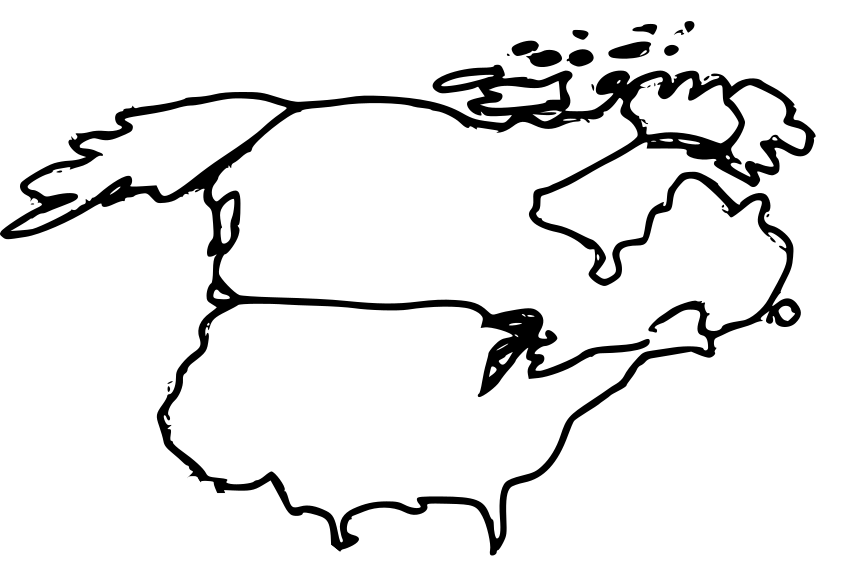
\includegraphics[width=1.5\textwidth]{imgs/usa.png}};
        %
        \draw[<-,ultra thick] ($(usa)+(1.9,-0.7)$) .. controls ($(usa)+(4.7,-0.4)$) .. ($(usa)+(5,0.1)$) node [above,align=center,font=\scriptsize] {\textbf{MIT}~\\ D. Bertsimas, R. Mazmuder, ...~\\\textit{MIO tools for $\ell_0$-problems}};
        %
        \draw[<-,ultra thick] ($(usa)+(0.25,0.45)$) .. controls ($(usa)+(-1.9,0.1)$) .. ($(usa)+(-2.3,-0.1)$) node [below,align=center,font=\scriptsize] {\textbf{Google Deep Mind}~\\ H. Hazimeh, A. Dedieu, ...~\\\textit{MIO-based heuristics and} \\ \textit{softwares}};
        %
        \draw[<-,ultra thick] ($(usa)+(-0.5,-1.2)$) .. controls ($(usa)+(-1.5,-1.4)$) .. ($(usa)+(-2,-1.9)$) node [below,align=center,font=\scriptsize] {\textbf{Berkley}~\\ A. Atamtürk, A. Gomès, ...~\\\textit{Convex-based acceleration}};
        %
        %
        %
        \node[align=center,text width=0.3\linewidth] (europe) at ($(current page.center)+(3.75,-2.5)$) {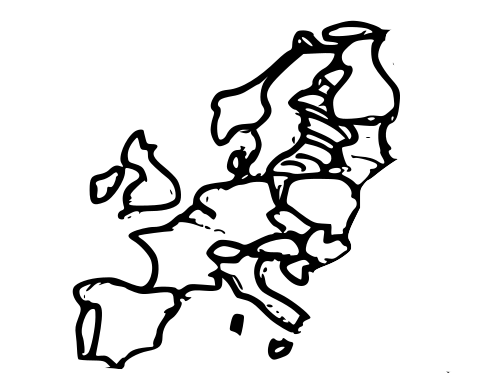
\includegraphics[width=1.5\textwidth]{imgs/europe.png}};
        %
        \draw[<-,ultra thick] ($(europe)+(0.7,1)$) .. controls ($(europe)+(0.5,1.5)$) .. ($(europe)+(1.1,3.5)$) node [above,align=center,font=\scriptsize] {\textbf{Lund University}~\\ M. Carlsson, C. Olsson...~\\\textit{Quadratic envelope}};
        %
        \draw[<-,ultra thick] ($(europe)+(0.4,0.1)$) .. controls ($(europe)+(-0.5,1.5)$) .. ($(europe)+(-1.2,2.5)$) node [above,align=center,font=\scriptsize] {\textbf{Frankfurt / Wurzburg Universities}~\\ C. Kanzow, A. Tillmann, ...~\\\textit{Optimality conditions}};
        %
        \draw[<-,ultra thick] ($(europe)+(-0.4,0.5)$) .. controls ($(europe)+(-1,1.3)$) .. ($(europe)+(-2,1.5)$) node [above left,align=center,font=\scriptsize] {\textbf{London Business School}~\\ J. Pauphilet, R. Cory-Wright, ...~\\\textit{Healthcare applications}};
        %
        \draw[<-,ultra thick] ($(europe)+(0.2,-0.6)$) .. controls ($(europe)+(-1.5,0.8)$) .. ($(europe)+(-2.5,0.9)$) node [left,align=center,font=\scriptsize] {\textbf{Ponts ParisTech}~\\ M. De Lara, P. Chancelier, A. Parmentier, ...~\\\textit{Non-convex analysis for $\ell_0$-norm, ML appli.}};
        %
        \draw[<-,ultra thick] ($(europe)+(-0.4,-0.4)$) .. controls ($(europe)+(-1,-0.4)$) .. ($(europe)+(-5,-0.2)$) node [left,align=center,font=\scriptsize] {\textbf{Centrale Nantes / ENSTA Bretagne}~\\ S. Bourguignon, J. Ninin, ...~\\\textit{Branch-and-Bound for $\ell_0$-problems}};
        %
        \draw[<-,ultra thick] ($(europe)+(-0.2,-0.7)$) .. controls ($(europe)+(-4,-0.7)$) .. ($(europe)+(-5.7,-0.9)$) node [below left,align=center,font=\scriptsize] {\textbf{Inria / CentraleSupélec}~\\ C. Herzet, C. Elvira, A. Arslan, ...~\\\textit{Generalization, acceleration}};
        %
        \draw[<-,ultra thick] ($(europe)+(0,-0.9)$) .. controls ($(europe)+(-0.5,-1.5)$) .. ($(europe)+(-1.7,-1.5)$) node [left,align=center,font=\scriptsize] {\textbf{IRIT / I3S}~\\ E. Soubies, L. Blanc-Féraud, ...~\\\textit{Strong relax. of $\ell_0$-norm}};
    \end{tikzpicture}
\end{frame}
\begin{frame}{}
  \begin{tikzpicture}[remember picture,overlay]
    \node at ($(current page.north)+(0,-2)$) {\Large\textbf{\emphcolor{Brown}{Take-home message}}};
    \node[align=left,text width=1.1\textwidth] at ($(current page.north)+(0,-5.5)$) {
      \begin{itemize}
        \item[$\bullet$] In \emphcolor{Brown}{some} cases, solving $\ell_0$-norm problems \emphcolor{Brown}{exactly} worths-it
        \item[$\bullet$] There exists \emphcolor{Brown}{Mixed-Integer Optimization} tools to do so
        \item[$\bullet$] \emphcolor{Brown}{Structure exploitation} is the key to achieve competitive performances
        \item[$\bullet$] Active research area
        \begin{itemize}
          \item[$\rightarrow$] Theoretical results
          \item[$\rightarrow$] Efficiency, flexibility and accessibility of solution methods
          \item[$\rightarrow$] Software development
          \item[$\rightarrow$] Diffusion to other communities
        \end{itemize}
      \end{itemize}
    };
  \end{tikzpicture}
\end{frame}
\begin{frame}[standout]
    \begin{tikzpicture}[remember picture,overlay]
        \node[align=center] at ($(current page.center)+(0,-0)$) {Question time \\~\\ 
\includegraphics[width=30pt]{imgs/nerd_face.png}};
        % \node at ($(current page.north)+(0,-5)$) {
        %     
\includegraphics[width=30pt]{imgs/nerd_face.png}
        % };  
    \end{tikzpicture}
\end{frame}

\section{Supplementary Slides}

\begin{frame}[noframenumbering]{Lower bounding}
    \begin{tikzpicture}[remember picture,overlay]
        \onslide<+-> {
            \node at ($(current page.north)+(-4.5,-0.325\textheight)$) (node) {};
            \draw[
                ultra thick,
                top color = white,
                bottom color = blue!30,
            ] (node) circle (15pt) node {\Large$\nodeSymbIter{}_k$};
            \draw[ultra thick,->] ($(node.north)+(0,0.75)$) -- ($(node.north)+(0,0.4)$);
            \node at ($(node.south)+(0,-0.75)$) (nodesets) {$(\setzero,\setone)$};
            %
            \node[text width=.5\textwidth] at ($(current page.north)+(0,-0.3\textheight)$) (nodeproblem) {
                \begin{blockcolor}{black}{Node problem}
                    \centering
                    \small
                    $\node{\pobj} = 
                        \left\{
                        \begin{array}{rl}
                            \min & \lossfunc(\pv) + \reg \transp{1}\bv + \pertfunc(\pv,\bv) \\
                            \text{s.t.} & \subzero{\bv} = \0, \ \subone{\bv} = \1
                        \end{array}
                        \right.
                    $
                \end{blockcolor}
            };
        }
        %
        %
        %
        \onslide<+-> {
            \draw[ultra thick,<-] ($(nodeproblem.east)+(0.1,-0.1)$) .. controls ($(nodeproblem.east)+(0.75,-0.1)$) .. ($(nodeproblem.east)+(1,-0.5)$) node[font=\small,below] {$\min_{\pv,\bv} \pfunc(\pv,\bv)$};
        }
        %
        %
        %
        \onslide<+-> {
            \node[text width=.44\textwidth] at ($(nodeproblem.south)+(0,-0.15\textwidth)$) (lbproblem) {
                \begin{blockcolor}{Brown}{Lower-bounding problem}
                    \centering
                    $\node{\LB{\pobj}} = \min_{\pv,\bv} \biconj{\pfunc}(\pv,\bv)$
                \end{blockcolor}
            };
            %
            \draw[ultra thick,->] ($(nodeproblem.south)+(0,0)$) -- ($(lbproblem.north)+(0,-0.3)$) node[midway,draw,fill=white,font=\small] {Bi-conjugacy $\biconj{\pfunc}(\pv,\bv) \leq \pfunc(\pv,\bv)$};
        }
        %
        %
        %
        \onslide<+-> {
            \node[font=\small] (issue) at ($(lbproblem.south)+(0,-0.1\textwidth)$) {\textbf{Bi-conjugate computation is also NP-hard}};
            \draw[ultra thick,->] ($(lbproblem.south)+(0,-0.05)$) -- ($(issue.north)+(0,+0.1)$);
            \node at ($(issue)+(0,-0.75)$) {
                
\includegraphics[width=20pt]{imgs/dizzy.png}
            };
        }
    \end{tikzpicture}
\end{frame}

\begin{frame}[noframenumbering]{Graphical intuition}
    \newcommand{\pointsize}{0.03}
    \begin{tikzpicture}[
        remember picture,
        overlay,
        domain=-0.8:0.8,
    ]
        \begin{scope}[shift={(2,0)},xscale=2.3,yscale=2.5]
            \node (origin) at (0,0) {};
            \draw[ultra thick,->] (-1,0) -- (1, 0);
            \draw[ultra thick,->] (0,0) -- (0, 1);
            \draw[ultra thick] (-0.03,0.2) -- (0.03,0.2);
            \node[above right] at (0,0.2) {$\reg$};
            \node[right] at (1,0) {$\pv$};
            \node[above] at (0,1) {\small\textcolor{Teal}{$\pertfunc(\pv,\bv) \equiv$ Big-M}};
            %
            \draw[{Arc Barb[arc=130,reversed]}-,Teal,ultra thick] (-0.5,0.2) plot[domain=0.03:0.5] (\x,0.2);
            \draw[-{Arc Barb[arc=130,reversed]},Teal,ultra thick] (-0.5,0.2) plot[domain=-0.5:-0.03] (\x,0.2) node {};
            \fill[Teal] (0,0) circle (\pointsize);
            \fill[Teal] (-0.5,0.2) circle (\pointsize);
            \fill[Teal] (0.5,0.2) circle (\pointsize);
            \draw[dashed,Teal,ultra thick] (0.5,0.2) -- (0.5,0.85);
            \draw[dashed,Teal,thick] (-0.5,0.2) -- (-0.5,0.85);
            %
            %
            %
            \draw[ultra thick,densely dashed] (0, 0) -- (1, 0.4);
            %
            %
            %
            \draw[ultra thick] (0.5,-0.03) -- (0.5,0.03);
            \node[below] at (0.5,0) {\small{$\pertlimit$}};
            \draw[ultra thick,densely dashed] (0.5,0) -- (0.5,0.2);
            \node[rotate=25,anchor=center] at (0.8,0.25) {\scriptsize{slope $\pertslope$}};
            %
            %
            %
            \draw[Brown,ultra thick] (0, 0) -- (0.5, 0.2);
            \fill[Teal] (0,0) circle (\pointsize);
            \fill[Teal] (0.5,0.2) circle (\pointsize);
            %
            %
            %
            \draw[dashed,Brown,ultra thick] (0.51,0.2) -- (0.51,0.85);
            \fill[Teal] (0.5,0.2) circle (\pointsize);
            %
            %
            %
            \draw[Brown,ultra thick] (0, 0) -- (-0.5, 0.2);
            \draw[dashed,Brown,ultra thick] (-0.51,0.2) -- (-0.51,0.85);
            \draw[ultra thick] (-0.5,-0.03) -- (-0.5,0.03);
            \node[below] at (-0.5,0) {\small{$-\pertlimit$}};
            \fill[Teal] (0,0) circle (\pointsize);
            \fill[Teal] (-0.5,0.2) circle (\pointsize);
            %
            %
            %
            \draw[ultra thick,<-,Brown] (-0.2,0.07) .. controls (-0.2,-0.15) .. (-0.05,-0.2) node[right] {\small\emphcolor{Brown}{$\biconj{\regfunc}(\pv)$}};
        \end{scope}
        %
        %
        %
        \begin{scope}[shift={(8,0)},xscale=2.3,yscale=2.5]
            \node (origin) at (0,0) {};
            \draw[ultra thick,->] (-1,0) -- (1, 0);
            \draw[ultra thick,->] (0,0) -- (0, 1);
            \draw[ultra thick] (-0.03,0.2) -- (0.03,0.2);
            \node[above right] at (0,0.2) {$\reg$};
            \node[right] at (1,0) {$\pv$};
            \node[above] at (0,1) {\small\textcolor{Teal}{$\pertfunc(\pv,\bv) \equiv$ L2-norm}};
            \draw[{Arc Barb[arc=130,reversed]}-,Teal,ultra thick] (-0.5,0.2) plot[domain=0.03:0.8] (\x,0.2+\x^2);
            \draw[-{Arc Barb[arc=130,reversed]},Teal,ultra thick] (-0.5,0.2) plot[domain=-0.8:-0.03] (\x,0.2-\x^2) node {};
            \fill[Teal] (0,0) circle (\pointsize);
            %
            %
            %
            \draw[ultra thick,densely dashed] (0, 0) -- (1, 0.86);
            %
            %
            %
            \node[below] at (0.5,0) {\small{$\pertlimit$}};
            \draw[ultra thick,densely dashed] (0.5,0) -- (0.5,0.42);
            %
            %
            %
            \node[rotate=45,anchor=center] at (0.28,0.17) {\scriptsize{slope $\pertslope$}};
            %
            %
            %
            \draw[Brown,ultra thick] (0, 0) -- (0.5, 0.43);
            %
            %
            %
            \draw[Brown,ultra thick] (0.5, 0.43) plot[domain=0.5:0.8] (\x,0.2+\x^2-0.02) node {};
            %
            %
            %
            \draw[Brown,ultra thick] (0, 0) -- (-0.5, 0.43);
            \draw[Brown,ultra thick] (-0.5, 0.43) plot[domain=-0.8:-0.5] (\x,0.2-\x^2-0.02) node {};
            \fill[Teal] (0,0) circle (\pointsize);
            %
            \draw[ultra thick] (-0.5,-0.03) -- (-0.5,0.03);
            \node[below] at (-0.5,0) {\small{$-\pertlimit$}};
            \draw[ultra thick] (0.5,-0.03) -- (0.5,0.03);
            %
            %
            %
            \draw[ultra thick,<-,Brown] (-0.2,0.14) .. controls (-0.2,-0.15) .. (-0.05,-0.2) node[right] {\small\emphcolor{Brown}{$\biconj{\regfunc}(\pv)$}};
        \end{scope}
        %
        %
        %
        \node[text width=.5\textwidth] at ($(current page.north)+(0,-0.675\textwidth)$) (closedform) {
            \begin{blockcolor}{black}{Bi-conjugate closed-form}
                \small
                \centering
                $\biconj{\regfunc}(\pv) = 
                \begin{cases}
                    \emphcolor{Brown}{\pertslope}\abs{\pv} & \text{if} \ \abs{\pv} \leq \emphcolor{Brown}{\pertlimit} \\
                    \reg + \pertfunc(\pv,1) & \text{otherwise}
                \end{cases}$
            \end{blockcolor}
        };
    \end{tikzpicture}
\end{frame}

\begin{frame}[noframenumbering]{Overview of numerical performances}
    \begin{tikzpicture}[remember picture,overlay]
        \node [text width=.425\textwidth] at ($(current page.north)+(0,-0.175\textheight)$) (problem) {
            \begin{blockcolor}{black}{}
                \centering
                \small
                $\min_{\pv} \ \lossfunc(\pv) + \reg \transp{\1}\bv + \pertfunc(\pv,\bv)$
            \end{blockcolor}
        };
        %
        %
        %
        \node [text width=.7\textwidth] at ($(current page.north)+(2.3,-0.34\textheight)$) (data) {
          \begin{itemize}[nosep]
            \item[\textbf{Dataset}] : Sparse regression
            \item[\textbf{F($\cdot$)}] : Least-squares loss
            \item[\textbf{H($\cdot,\cdot$)}] : \emphcolor{Brown}{L2-norm}
            \item[$\boldsymbol{\lambda}$] : Set statistically
          \end{itemize}
        };
        \begin{scope}[shift={(0.75,-3)}]
        \begin{axis}[
            mlineplot,
            width = 0.6\textwidth,
            height = 5cm,
            xmode = log,
            xmin = 0.05,
            xmax = 5000,
            ymax = 1.1,
            xlabel = Time (seconds),
            ylabel =  Prop. solved within 1h,
            legend style={at={(1.03,0.5)},anchor=west}
        ]

        \addplot[ultra thick, smooth, color=RoyalBlue2] %
        table[x=times,y=Scip,col sep=comma]{data/perfprofiles_medium_Leastsquares_BigmL2norm_3600.csv};
        \addlegendentry{Scip};

        \addplot[ultra thick, smooth, color=SkyBlue2] %
        table[x=times,y=Cplex,col sep=comma]{data/perfprofiles_medium_Leastsquares_BigmL2norm_3600.csv};
        \addlegendentry{Cplex};

        \addplot[ultra thick, smooth, color=PaleGreen3] %
        table[x=times,y=Mosek,col sep=comma]{data/perfprofiles_medium_Leastsquares_BigmL2norm_3600.csv};
        \addlegendentry{Mosek};

        \addplot[ultra thick, smooth, color=DarkGoldenrod1] %
        table[x=times,y=L0Bnb,col sep=comma]{data/perfprofiles_medium_Leastsquares_BigmL2norm_3600.csv};
        \addlegendentry{L0Bnb (Hazimeh et al., 2022)};

        \addplot[ultra thick, smooth, color=Firebrick4] %
        table[x=times,y=El0ps,col sep=comma]{data/perfprofiles_medium_Leastsquares_BigmL2norm_3600.csv};
        \addlegendentry{El0ps (Guyard et al., 2023)};
        \end{axis}
        \end{scope}
      \end{tikzpicture}
\end{frame}

\begin{frame}[noframenumbering]{Overview of numerical performances}
    \begin{tikzpicture}[remember picture,overlay]
        \node [text width=.425\textwidth] at ($(current page.north)+(0,-0.175\textheight)$) (problem) {
            \begin{blockcolor}{black}{}
                \centering
                \small
                $\min_{\pv} \ \lossfunc(\pv) + \reg \transp{\1}\bv + \pertfunc(\pv,\bv)$
            \end{blockcolor}
        };
        %
        %
        %
        \node [text width=.7\textwidth] at ($(current page.north)+(2.3,-0.34\textheight)$) (data) {
          \begin{itemize}[nosep]
            \item[\textbf{Dataset}] : \emphcolor{Brown}{Sparse classification}
            \item[\textbf{F($\cdot$)}] : \emphcolor{Brown}{Logistic loss}
            \item[\textbf{H($\cdot,\cdot$)}] : L2-norm
            \item[$\boldsymbol{\lambda}$] : Set statistically
          \end{itemize}
        };
        \begin{scope}[shift={(0.75,-3)}]
        \begin{axis}[
            mlineplot,
            width = 0.6\textwidth,
            height = 5cm,
            xmode = log,
            xmin = 0.05,
            xmax = 5000,
            ymax = 1.1,
            xlabel = Time (seconds),
            ylabel = Prop. solved within 1h,
            legend style={at={(1.03,0.5)},anchor=west}
        ]

        \addplot[ultra thick, smooth, color=PaleGreen3] %
        table[x=times,y=Mosek,col sep=comma]{data/perfprofiles_medium_Logistic_Bigm_3600.csv};
        \addlegendentry{Mosek};

        \addplot[ultra thick, smooth, color=Firebrick4] %
        table[x=times,y=El0ps,col sep=comma]{data/perfprofiles_medium_Logistic_Bigm_3600.csv};
        \addlegendentry{El0ps (Guyard et al., 2023)};
        \end{axis}
        \end{scope}
      \end{tikzpicture}
\end{frame}

\end{document}